\chapter{Results and Discussion}
\label{resultanddiscussion}


This chapter covers the results and the discussion of all tests formulated in Chapter \ref{configurationandtesting}. In addition potentially needed optimization steps will be highlighted.
\section{Odometry test}

When looking at the odometry published by the differential drive plugin during the test in Figure \ref{wheel odom} it is noticeable, that the measurement has a huge rotational error, which is expected since the wheels always slip slightly when turning a differential drive robot.
\todo{picture including true odometry}
\begin{figure}[H]
	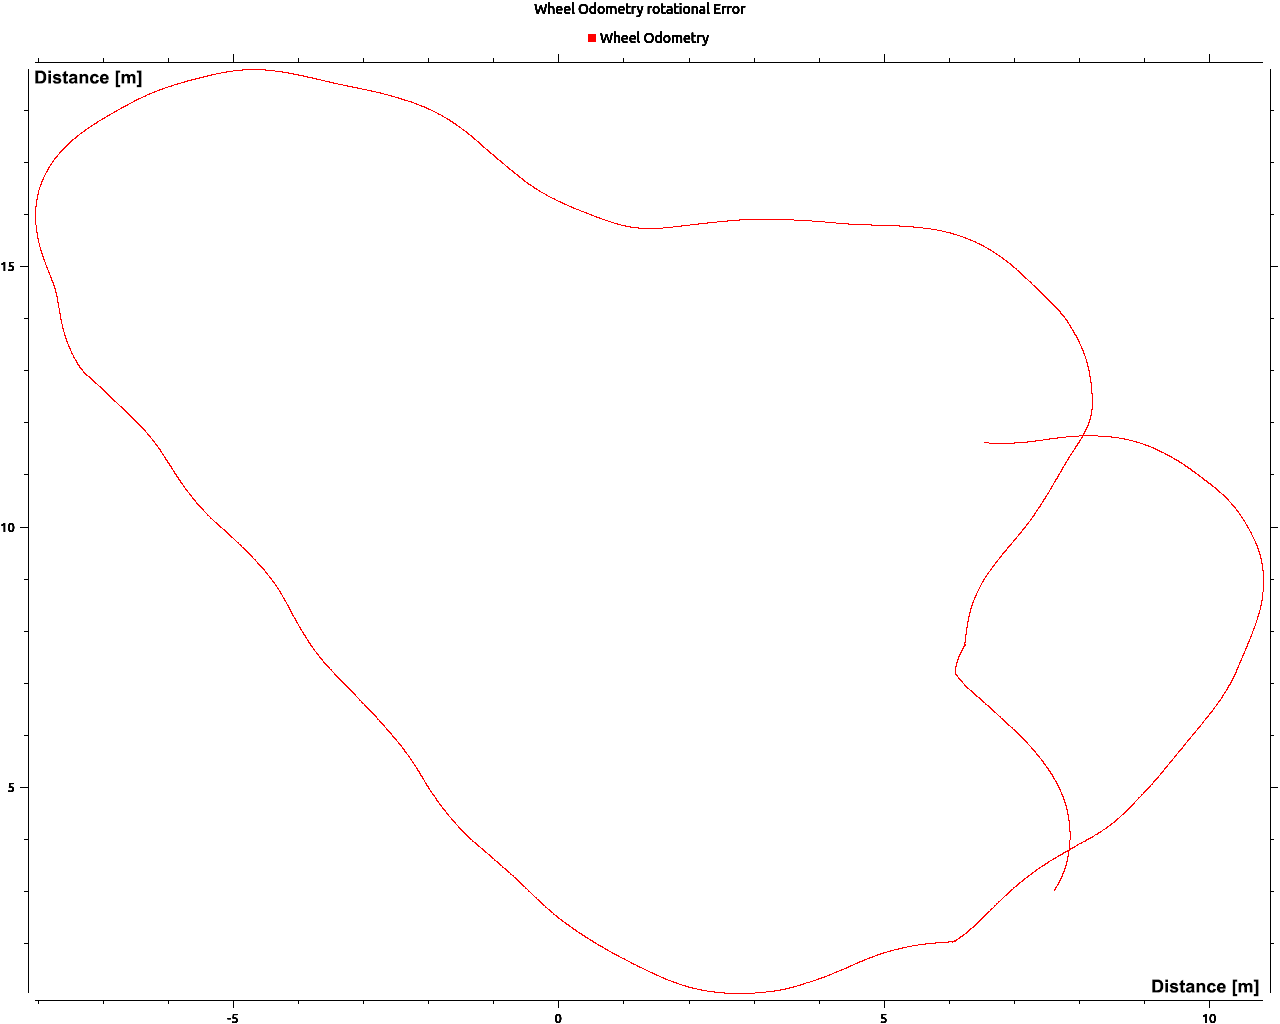
\includegraphics[width=\textwidth]{Pictures/rot error}
	\caption{Odometry Test result}
	\label{wheel odom}

\end{figure}

The quality of the odometry obviously is not sufficient and has to be improved.

\subsection{Optimization}
Since the odometry is found to not being sufficient for the navigation the following optimization approach will be tried and further testing will be performed. The test scenario will remain the same.

To improve the odometry the ROS package robot\_localization can be used. It provides an extended kalman filter for the fusion of sensor data for odometry.\\

To reduce the rotational error, an IMU (Inertia measurement unit) will be added to the robot configuration. Both, the imu and the wheel encoder will be fused by robot\_localization.

The IMU provides the following data:
\begin{itemize}
	\item orientation
	\item angular velocity
	\item linear acceleration
\end{itemize}

In this usecase the IMU is only supposed to measure data relevant for 2D operation roll, pitch and tranlation in z (axis according to to REP 103) will not be passed to the filter. 

The IMU is used for localization purposes, therefore the linear acceleration data is not interesting, since the accelerations would need to be integrated twice to be used for the pose. This would amplify every little error in the measured acceleration and will decrease the reliability of the odometry with increasing time.\\

Accordingly the only things fused from the imu are the yaw orientation and velocity.\\

Just like the IMU data the integration of the wheel-odometry data has to be discussed which consist only from linear and angular velocities, aswell as a pose derived from the velocities.\\

Here the most interesting part is the y velocity since the robot is relying on differential drive steering and therefore not able to have instantaneous y acceleration other than drift.\\

In contrast to the acceleration values of the IMU the y velocity will be included since according to Tom Moore (the developer of robot\_localization) it will give certainty that the robot has not moved in the y direction\cite{robotlocalizationconfiguration}. Obviously the x and yaw velocity have to be included aswell.

The position component of the wheel-odometry on the other hand will not be used, based on the fact that the position is already derived from the velocitys this would include the same data twice.\\

Unfortunately this does not solve the problem of the odometry correction yet. As visible in Figure \ref{pose comparison wheel odom + IMU} the odometry of the extended kalman filter has large jumps in it compared to the wheel-odometry. When observing it in real time the ekf odometry starts to drift and jumps back after a certain amount of time.\\
Looking at the linear velocities of both the ekf and the wheel odometry in Figure \ref{velocity comparison wheel odom + IMU} it is noticeable that the ekf filter does estimate a continuous acceleration, whereas the velocity of the wheel encoders actually decreases.\\



\begin{figure}[H]
	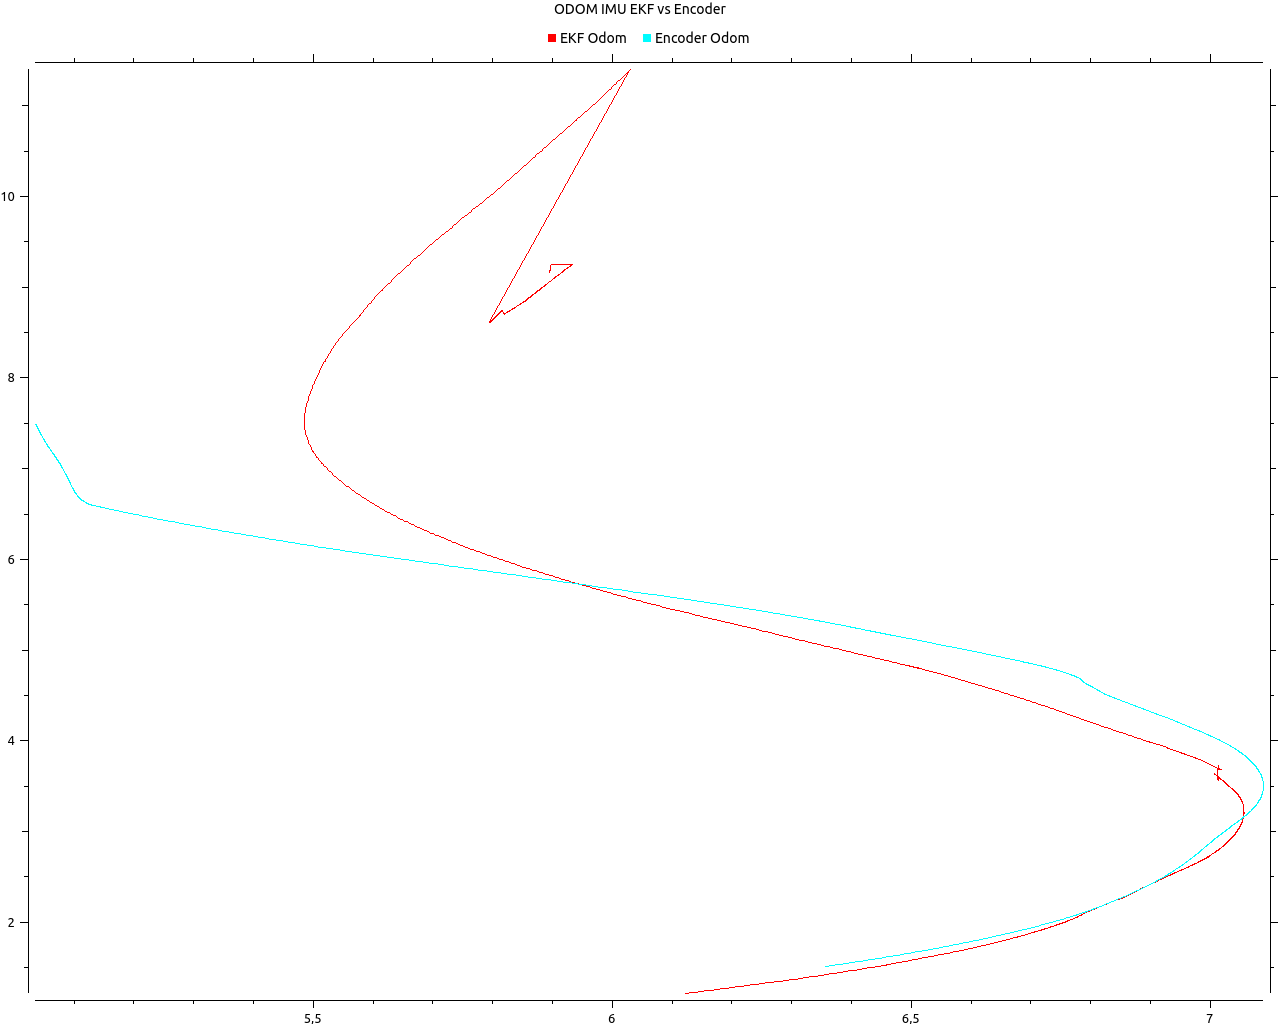
\includegraphics[width=\textwidth]{Pictures/odom pose comp}
	\caption{pose comparison wheel odom + IMU}
	\label{pose comparison wheel odom + IMU}

\end{figure}

\begin{figure}[H]
	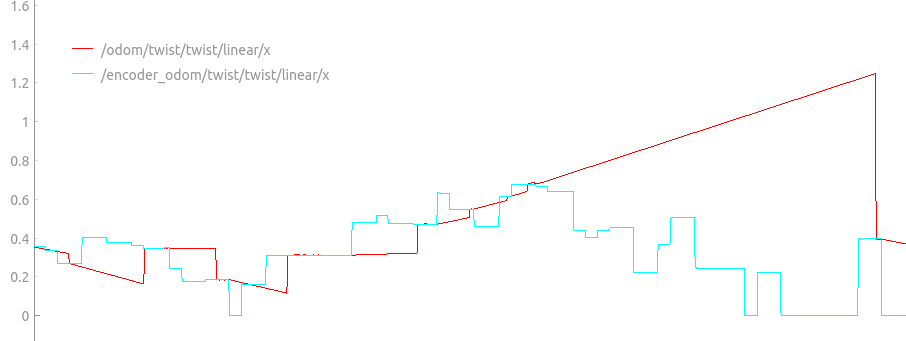
\includegraphics[width=\textwidth]{Pictures/comparison odom}
	\caption{velocity comparison wheel odom + IMU}
	\label{velocity comparison wheel odom + IMU}

\end{figure}


To fix this a logical approach is to include more data about the robots movement. Fortunately robot\_localization has an input for command velocities such as velocities produced by move base. While the command velocity does not provide any measurement in the real world the ekf filter can profit from knowing what the velocity actually should be.\\
It is very important to set the control timeout to a value that is larger than the cycle time of move\_base. Otherwise this will lead to translational offsets caused by too low estimate for the velocities like shown in Figure \ref{velocity offset}.

\begin{figure}[H]
	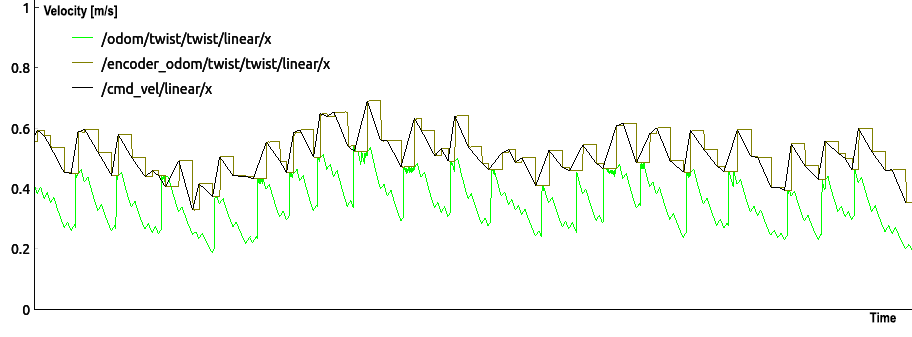
\includegraphics[width=\textwidth]{Pictures/velocity comp}
	\caption{velocity offset caused by too low control timout}
	\label{velocity offset}

\end{figure}


After the inclusion of the command velocity the acceleration limits in the configuration file of robot\_localization can be set equal to the limits in the local planner configuration.

When observing both the pose and velocities again it is noticeable, that the odometry has drastically improved as pictured in Figure \ref{Odometry comparison wheel odomIMUcmdvel}, equally the velocities stay closer together as pictured in \ref{velwithcmd}.

\begin{figure}[H]
	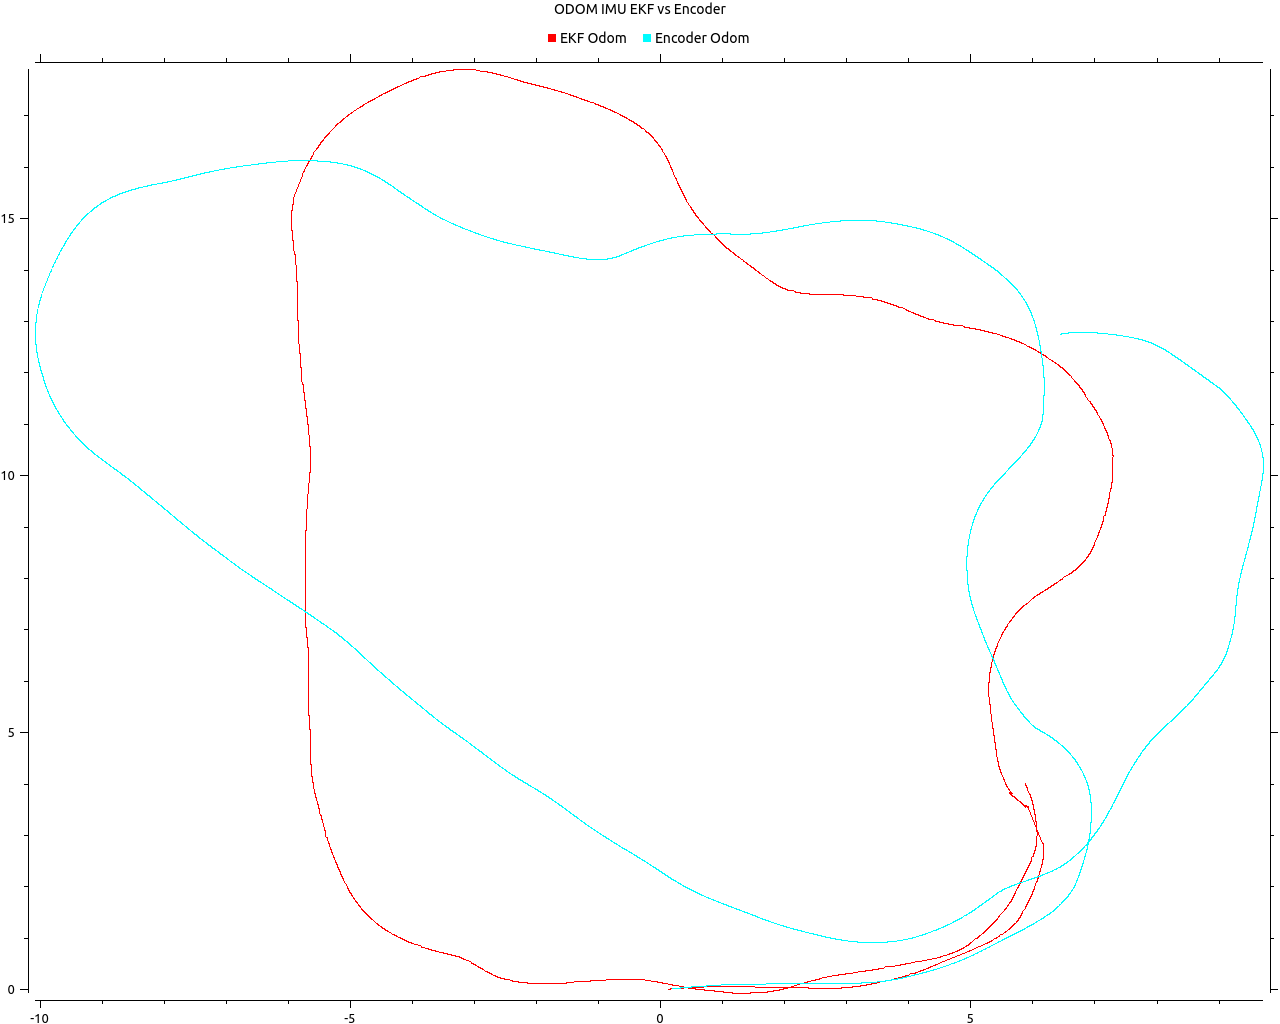
\includegraphics[width=\textwidth]{Pictures/odom after one round}
	\caption{Odometry comparison wheel odom + IMU + cmd\_vel}
	\label{Odometry comparison wheel odomIMUcmdvel}

\end{figure}
\begin{figure}[H]
	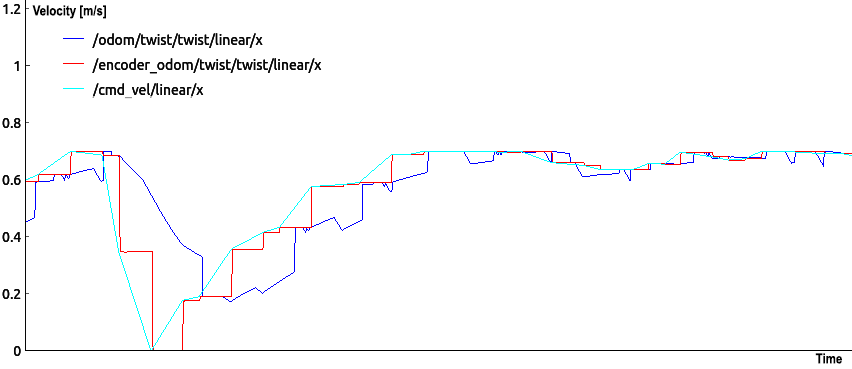
\includegraphics[width=\textwidth]{Pictures/circle vel}
	\caption{Velocity comparison with cmd\_vel}
	\label{velwithcmd}
\end{figure}



\begin{figure}[H]
	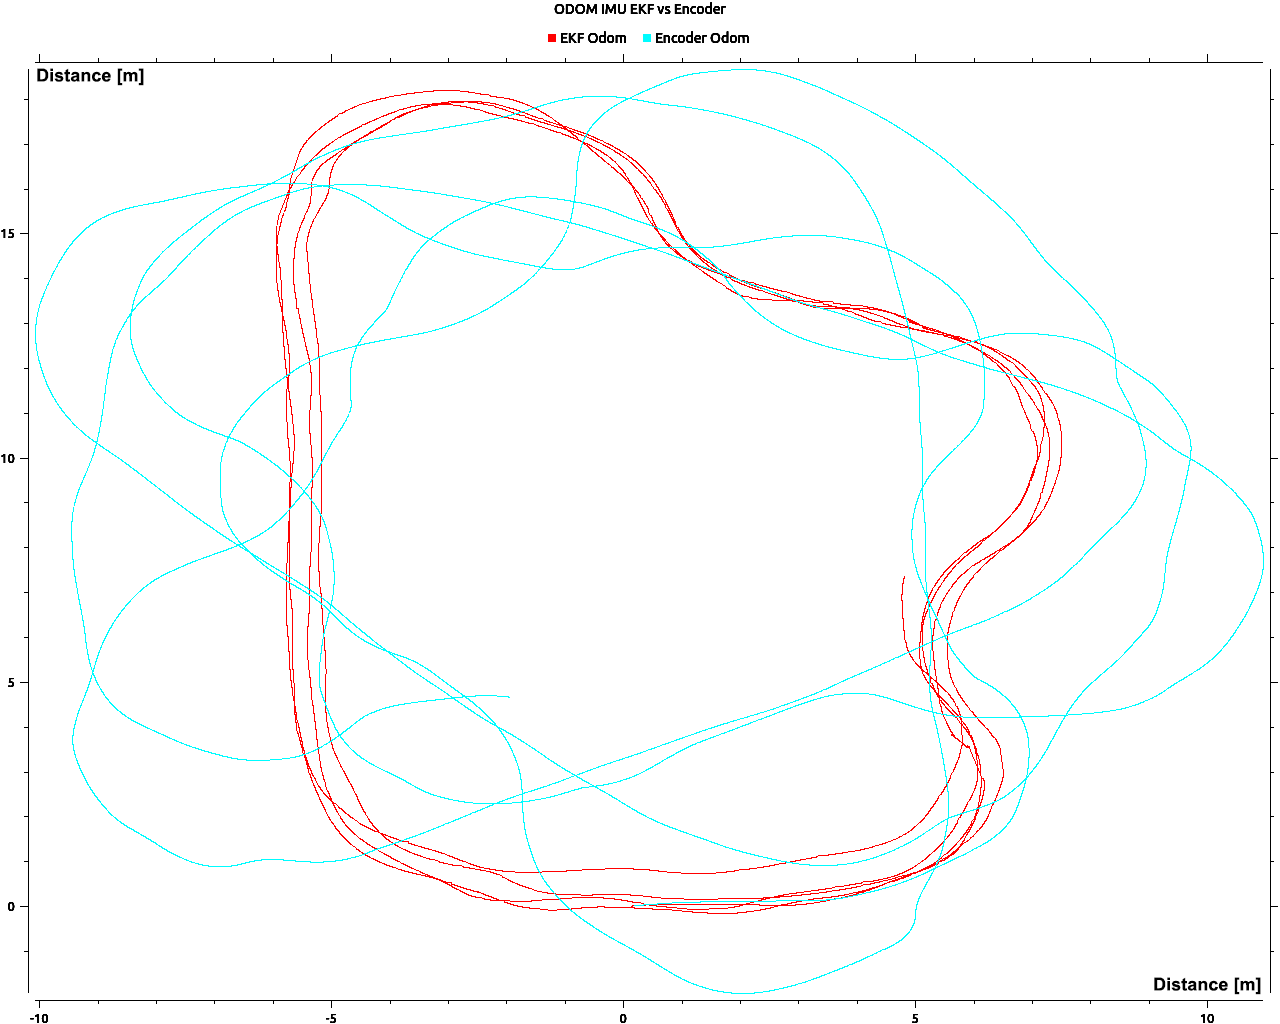
\includegraphics[width=\textwidth]{Pictures/odom comp multiple rounds}
	\caption{Odom comparison multiple rounds}
	\label{Odom comparison multiple rounds}

\end{figure}

Even after four rounds the odometry has not gained a large error in both translational and rotational as pictured in Figure \ref{Odom comparison multiple rounds}, furthermore the difference between the original odometry of the wheel encoders to the odometry from robot localization is quite remarkable.

After the rotantional and translational errors are marginal the scale of the odometry needs to be checked.
To isolate the different errors from the scaling error a circular track is build with a radius of 10 meter. Since the turning radius is constant this isolates the rotational error which can be seen at the graph of the wheel odometry in Figure \ref{circular track}.\\
The radius was chosen that high so potential errors are amplified and easier detectable.\\

Since the robot is driving on the lane and not on the middle road marking the expected radius is 10,45 meter. When evaluating the EKF odom in Figure \ref{circular track} we see that the scale is very precise.
 
\begin{figure}[H]
	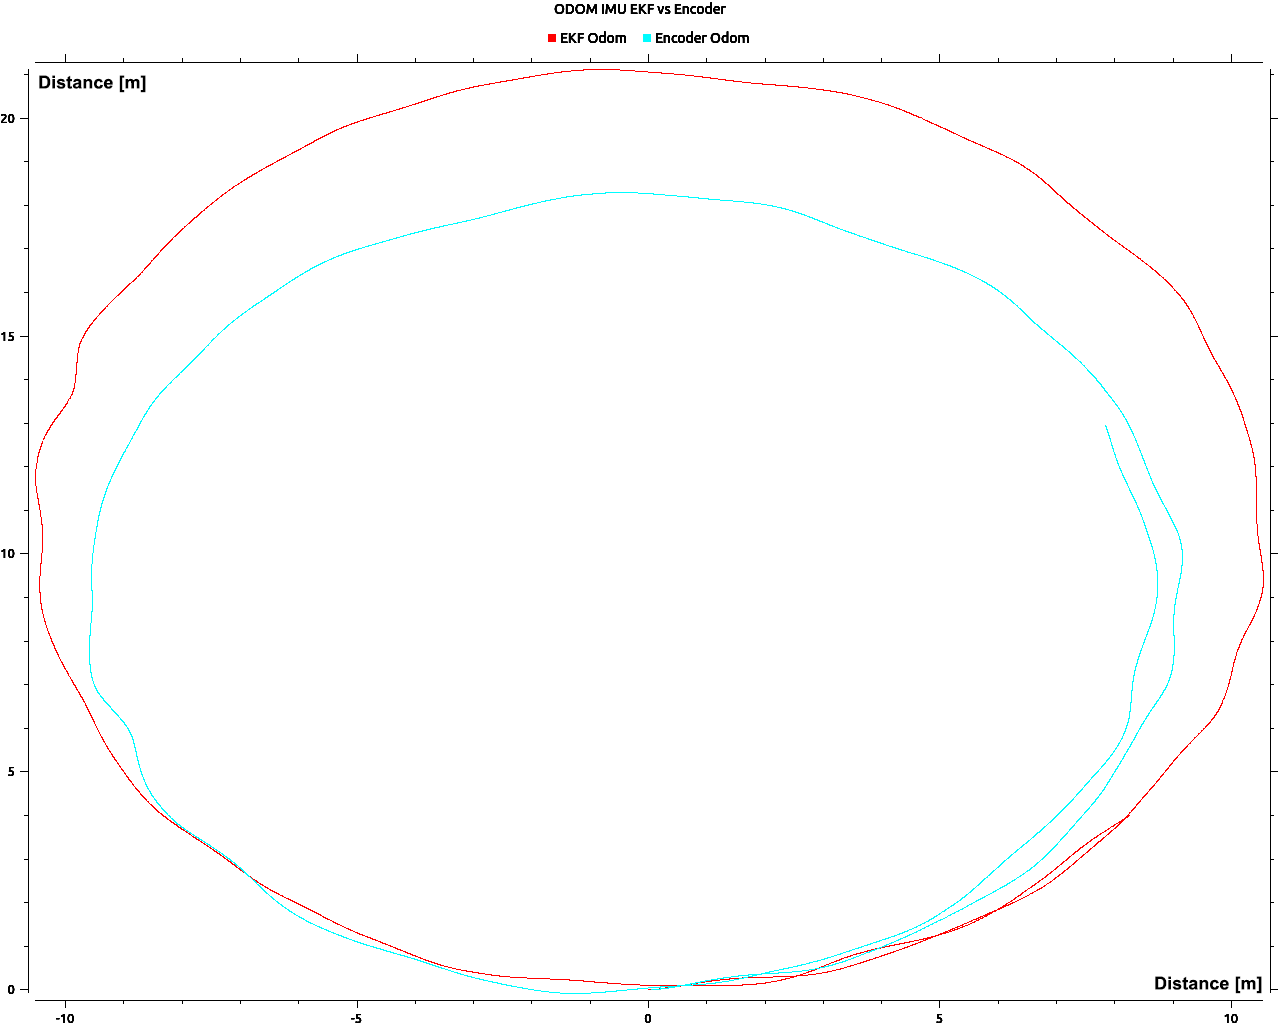
\includegraphics[width=\textwidth]{Pictures/circle odom}
	\caption{Odom comparison circular track}
	\label{circular track}

\end{figure}

As a final test the odometry from the robot\_localization node is compared to the true position from the simulation.

 \begin{figure}[H]
	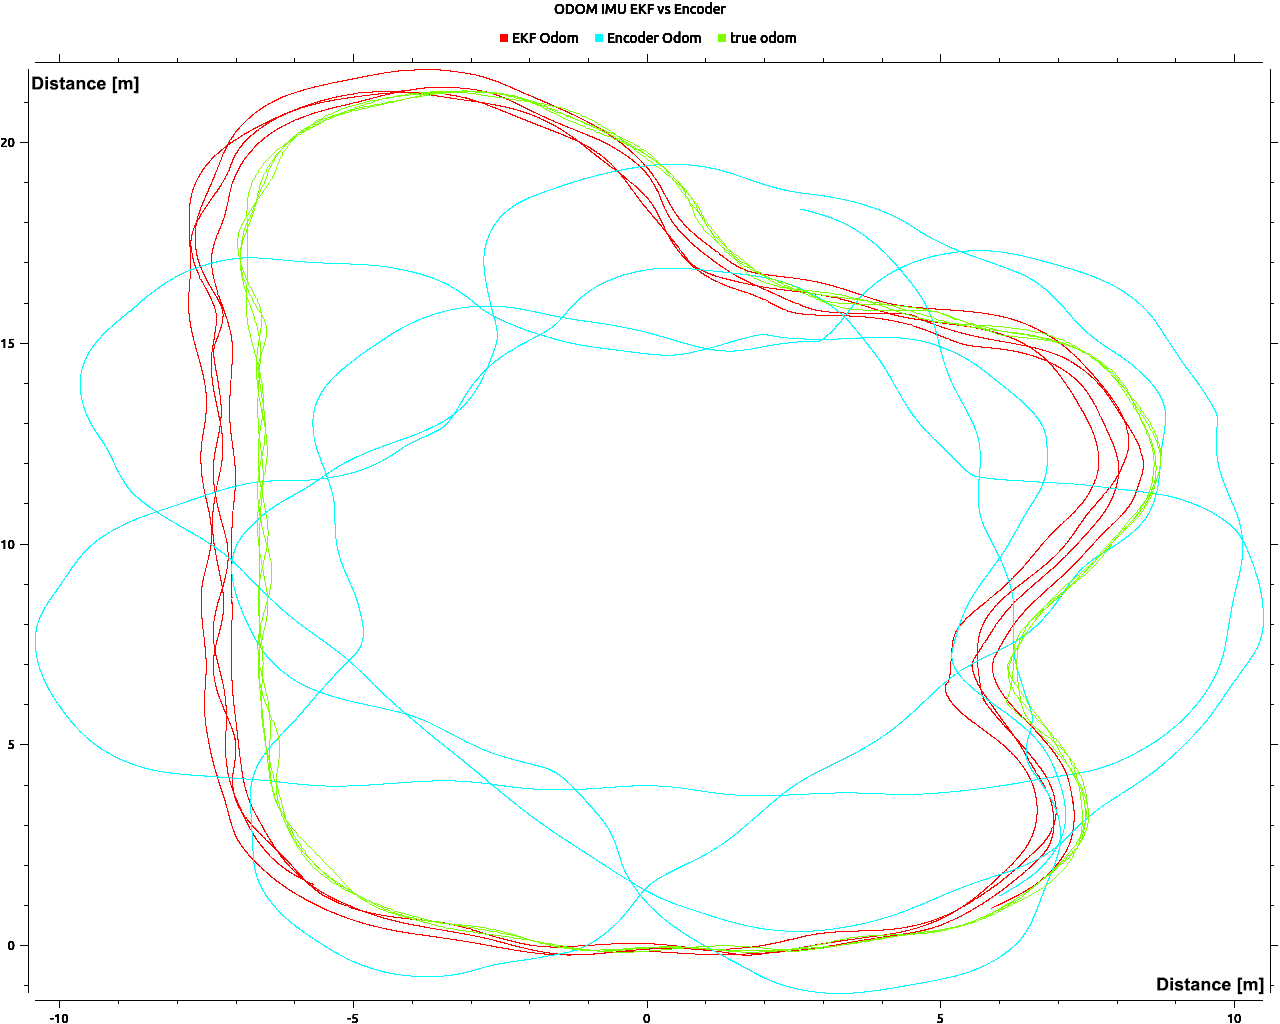
\includegraphics[width=\textwidth]{Pictures/odom with true}
	\caption{Comparison with true position}
	\label{trueodom}
\end{figure}

The comparison in Figure \ref{trueodom} shows, that the filtered odometry has a slight translational offset, but is very similar to the true odometry extracted from the simulation, hence it will be considered as sufficient for the navigation.


\section{Lidar test}


The Lidar sensor is simulated with realistic noise and errors. This also introduces the well known edge error in Laser distance measurement \cite{edgeeffect}. 

When using a ``realistic'' lidar to project obstacles into the costmap this error produces a lot of lethal point like obstacles that significately hinder navigation as visible in Figure \ref{unfiltered lidar}.

\begin{figure}[H]
	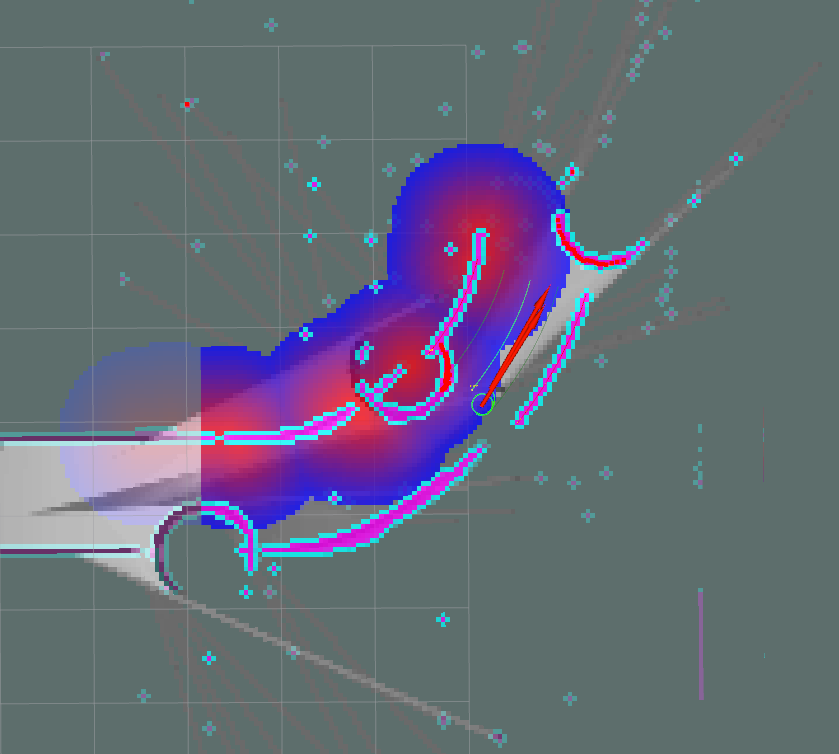
\includegraphics[width=\textwidth]{Pictures/Needs filtering of Laser}
	\caption{Lidar Test result}
	\label{unfiltered lidar}
\end{figure}

\subsection{Optimization}
To remove these error measurements the ROS package ``laser\_filters'' can be used. Among many different filter plugins that can be constructed into a filter chain it features the filter plugin ``ScanShadowFilter'' that is developed to remove the veiling effect around obstacles cause by the edge effect \cite{laserfilters}.


Figure \ref{lasercomp} shows a comparison between the filtered and not filtered laser scan, while keeping the data for 10 seconds. This allows to see the quickly jumping outliers caused by the edge effect. The filter seems well configured since the filtered points have no single outlier but still featuring a very good representation of the measured obstacle.

\begin{figure}[H]
	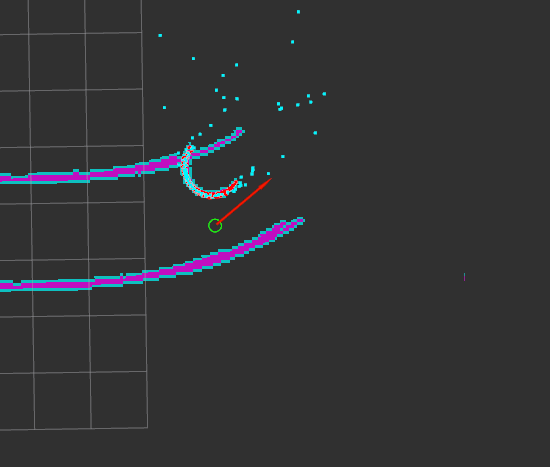
\includegraphics[width=\textwidth]{Pictures/LASERFILTER COMP}	
	\caption{comparison between filtered and not filtered laser scan (red - filtered, turquoise - raw)}
	\label{lasercomp}
\end{figure}

\section{road\_detection test}

As pictured in Figure \ref{longdurroad} the performance of the road detection converges to ca. 98.8\%. At the beginning the graph is not as reliable since there have not yet been enough measurements.\\

The duration of the test was roughly 1.5 hours of continuous navigation without obstacles in the simulation.

\begin{figure}[H]
	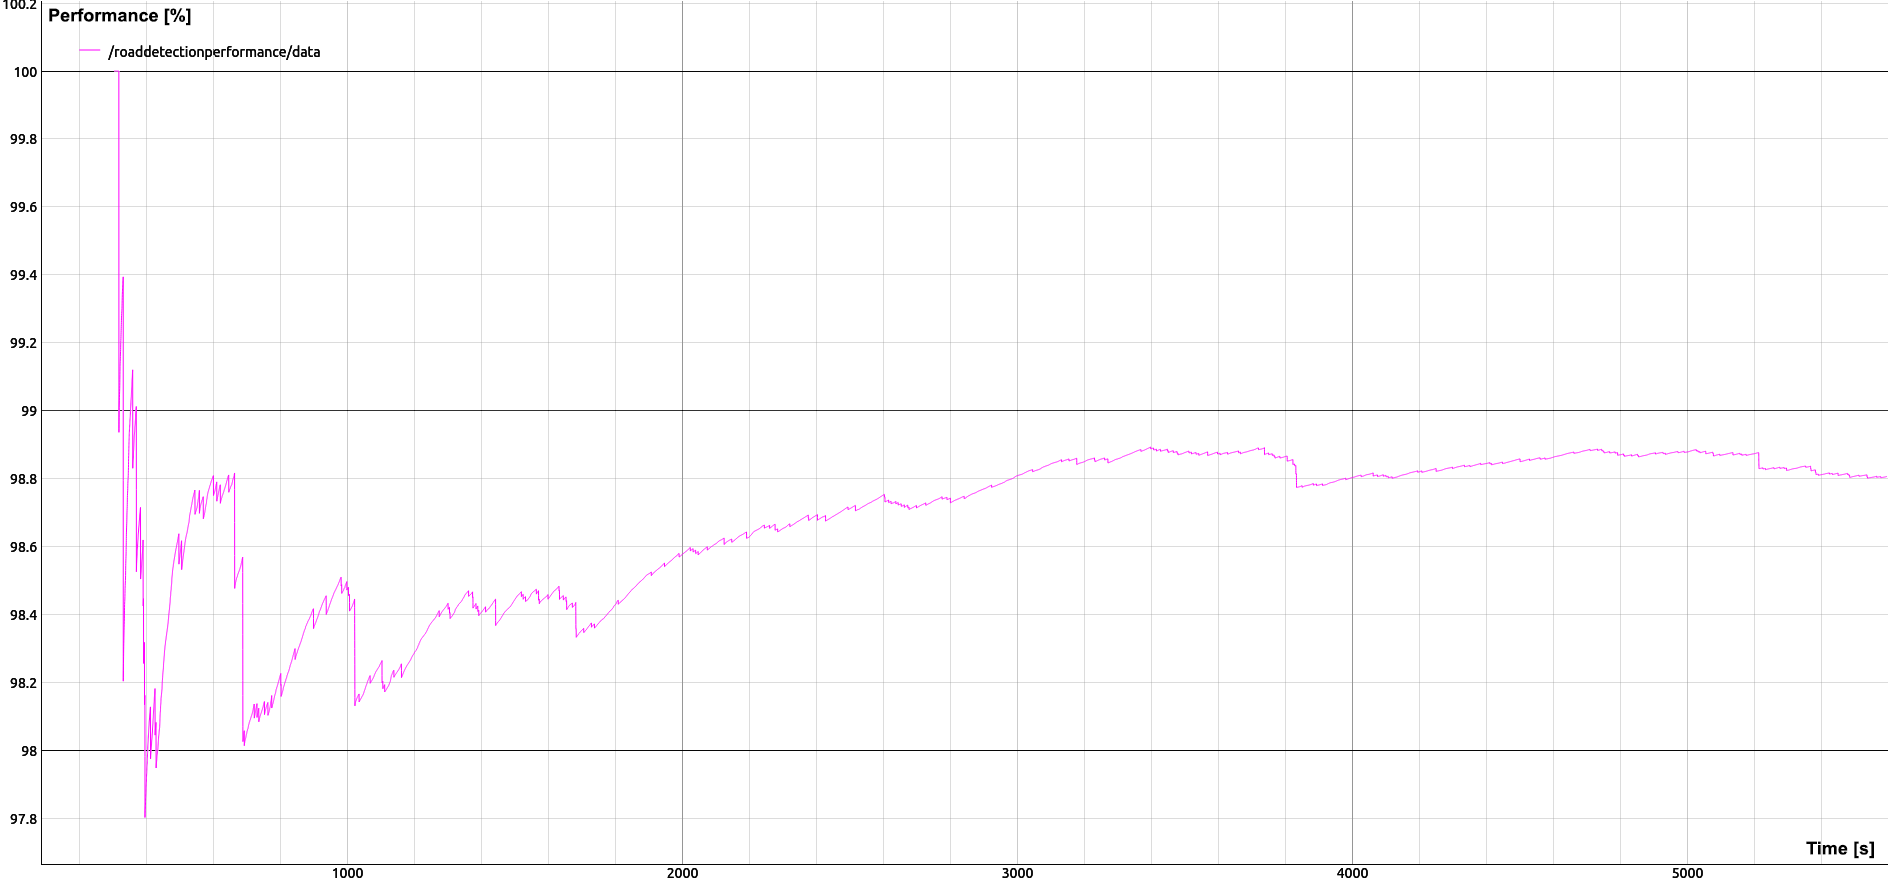
\includegraphics[width=\textwidth]{Pictures/long duration road detection test}
	\caption{roadRecordEvaluation during long duration test}
	\label{longdurroad}
\end{figure}

\section{SLAM test}
\textbf{Data purely from road detection:}\\

The following pictures contain the SLAM map after the \nth{1},\nth{2} and \nth{3} round.\\

\begin{figure}[H]
	\centering
	\begin{subfigure}{.3\linewidth}
		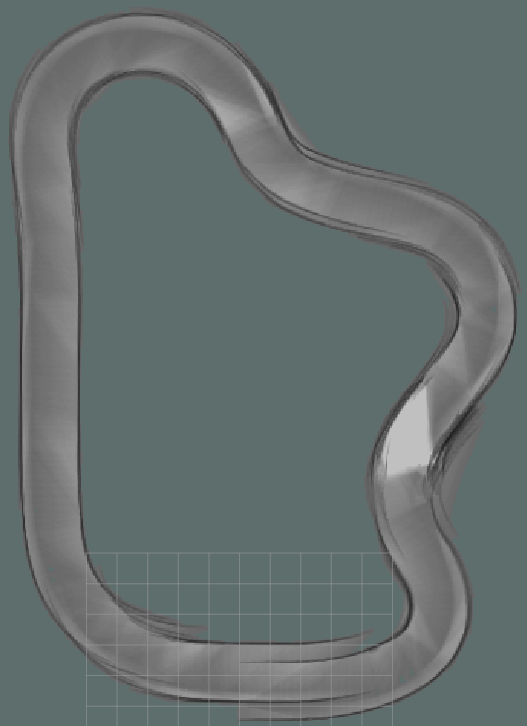
\includegraphics[width=\textwidth]{Pictures/1slamtest1}
		\caption{First}
		\end{subfigure}	
	%\hskip2em
	\begin{subfigure}{.3\linewidth}
		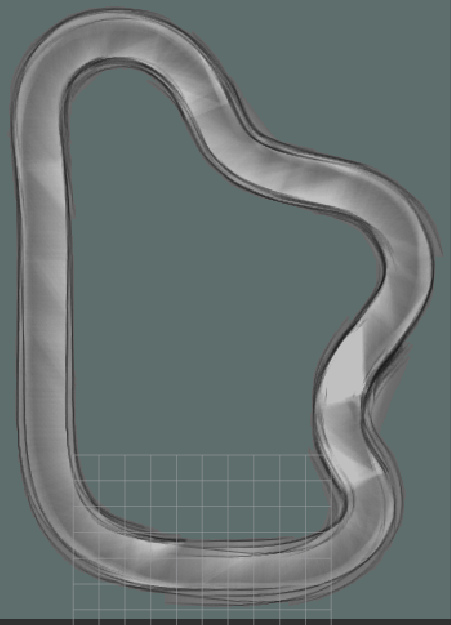
\includegraphics[width=\textwidth]{Pictures/1slamtest2}
		\caption{Second}
	\end{subfigure}
	%\hskip2em
	\begin{subfigure}{.3\linewidth}
		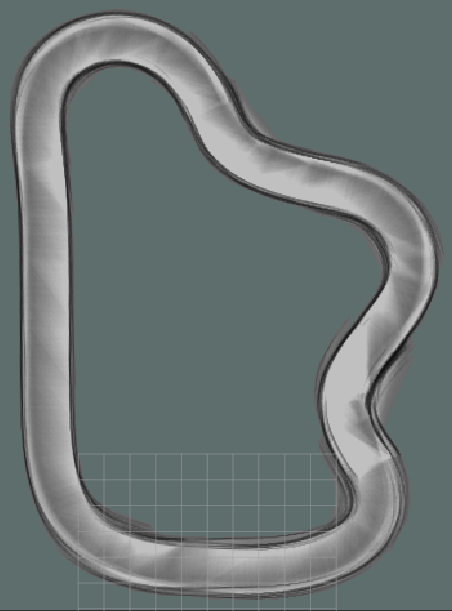
\includegraphics[width=\textwidth]{Pictures/1slamtest3}
		\caption{Third}
	\end{subfigure}

	\caption{Slam Map of first three rounds}
	\label{1slamtest}

\end{figure}

In the first round the map is not yet optimized. Like pictured in  Figure \ref{1slamtest} the road is not connected at the bottom after the first round, but has slight translational error.\\
In the second round the road is closed, but some submaps are slightly misaligned which can be seen by the blurry road markings.\\
This is well corrected in the third round and will improve from here on with every round, until the computational effort is too high.\\

\textbf{Data purely from localization and lidar scan with obstacles on the side of the road:}\\


As pictured in Figure \ref{2slamtest} cartographer manages to close the road already after the first round. After the second round the road borders are slightly blurry, therefore the submaps are not yet perfectly matched. This blurriness slightly improves after the third round, but the submaps are not yet perfectly matched with each other.

\begin{figure}[H]
	\centering
	\begin{subfigure}{.3\linewidth}
		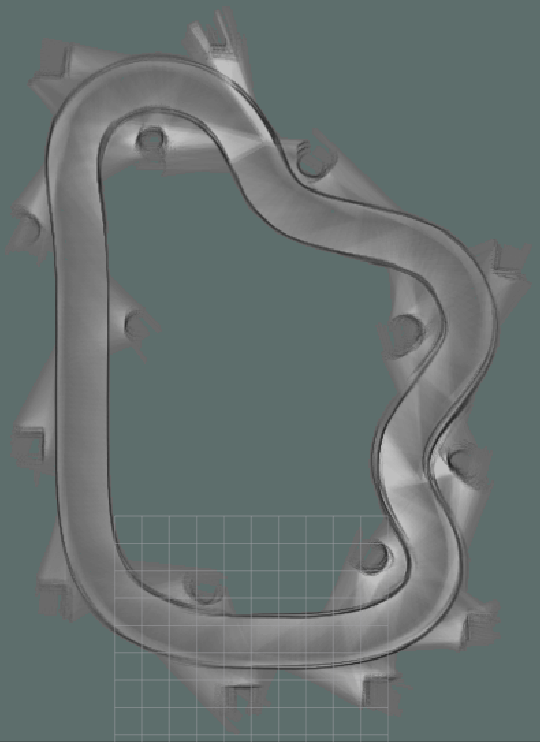
\includegraphics[width=\textwidth]{Pictures/2slamtest1}
		\caption{\nth{1} round}
		\end{subfigure}	
	%\hskip2em
	\begin{subfigure}{.3\linewidth}
		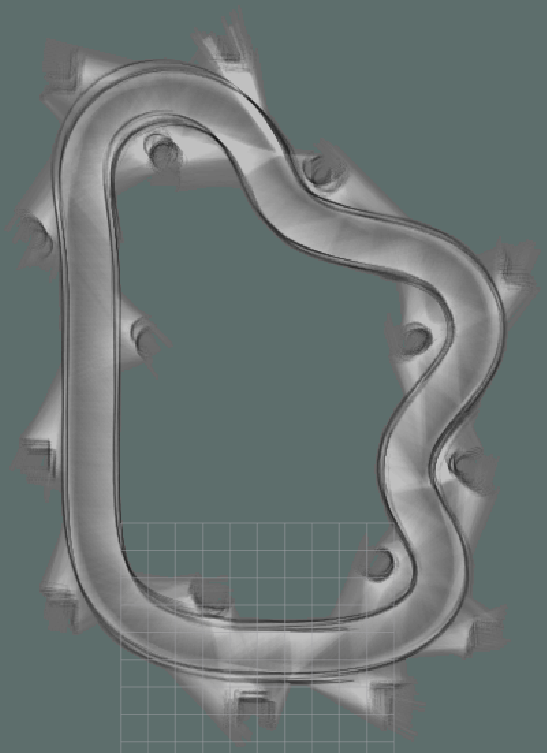
\includegraphics[width=\textwidth]{Pictures/2slamtest2}
		\caption{\nth{2} round}
	\end{subfigure}
	%\hskip2em
	\begin{subfigure}{.3\linewidth}
		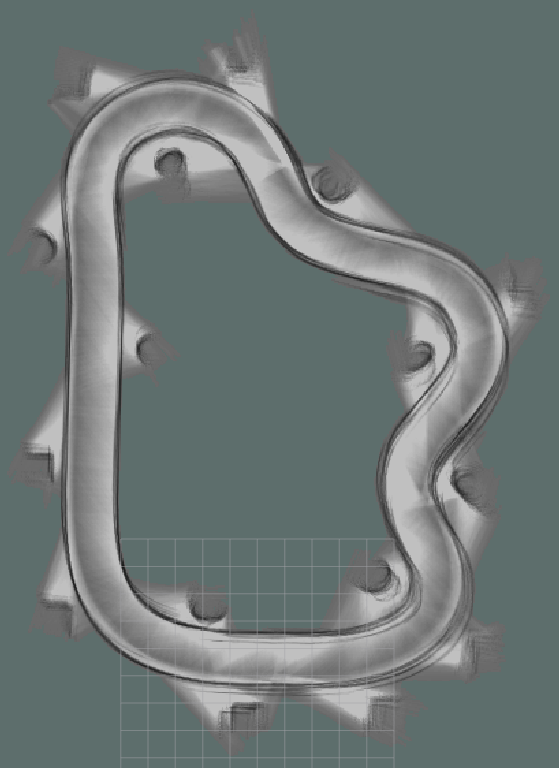
\includegraphics[width=\textwidth]{Pictures/2slamtest3}
		\caption{\nth{3} round}
	\end{subfigure}

	\caption{Slam Map of first three rounds}
	\label{2slamtest}

\end{figure}



\textbf{Long duration test with both road detection and lidar scan with obstacles on the side of the road:}\\

The map build by cartographer during this test (Figure \ref{3slamtest}) shows, that the map builds a very good representation of the real environment over the first four rounds.\\

After the \nth{7} round it is noticeable, that the matching of submaps seems to take more and more time, which is visible by a trace of unmatched submaps, that are slightly shifted. This is caused by the computational burden caused by the amount of submaps. In this round the cartographer node already takes up 20\% of the cpu resources and increases continuously. At this point realtime scan and submap matching is not possible anymore, resulting in enormous processing delays.

\begin{figure}[H]
	\centering
	\begin{subfigure}{.3\linewidth}
		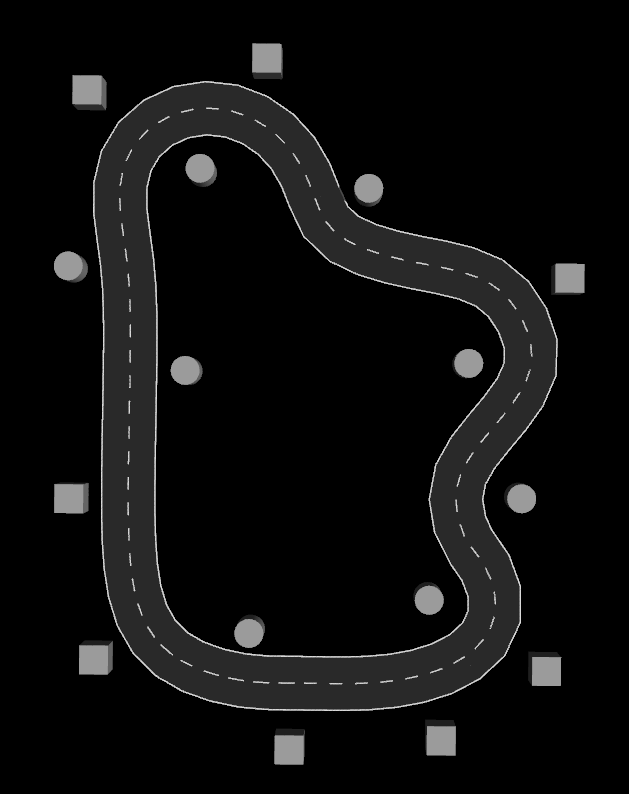
\includegraphics[width=\textwidth]{Pictures/2slamtest}
		\caption{Real Environment}
		\end{subfigure}	
	%\hskip2em
	\begin{subfigure}{.3\linewidth}
		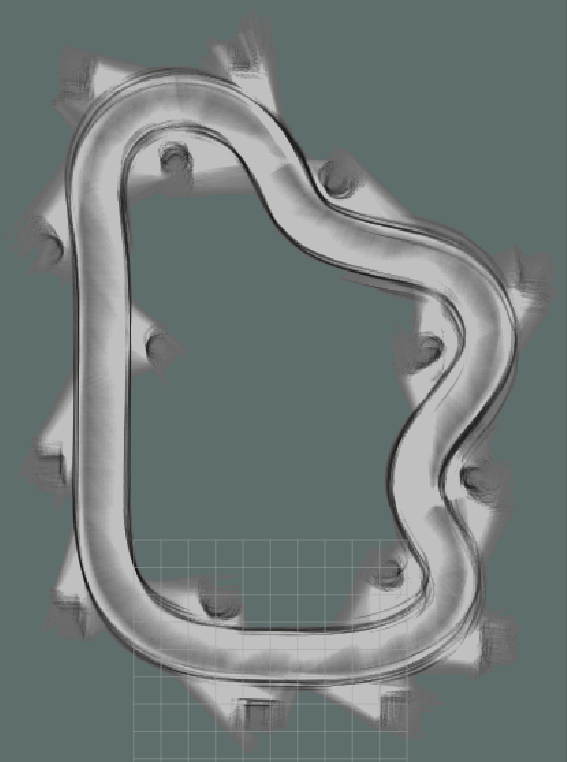
\includegraphics[width=\textwidth]{Pictures/2slamtest4}
		\caption{\nth{4} round}
	\end{subfigure}
	%\hskip2em
	\begin{subfigure}{.3\linewidth}
		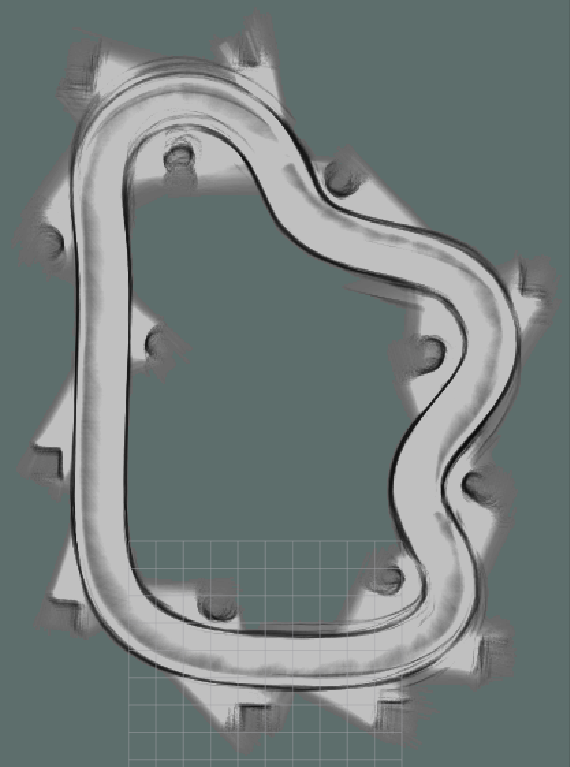
\includegraphics[width=\textwidth]{Pictures/2slamtest7}
		\caption{\nth{7} round}
	\end{subfigure}

	\caption{Slam Map rounds during long duration test}
	\label{3slamtest}

\end{figure}


\textbf{Data purely from localization and lidar scan with obstacles on the road:}\\

\begin{figure}[H]
	\centering
	\begin{subfigure}{.3\linewidth}
		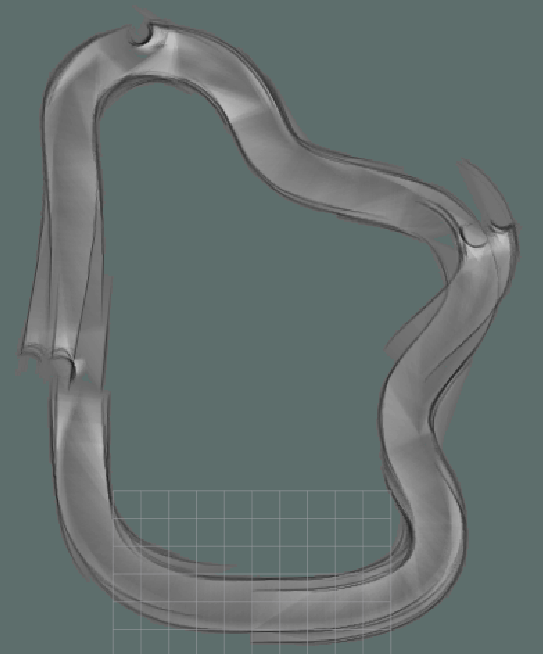
\includegraphics[width=\textwidth]{Pictures/3slamtest1}
		\caption{\nth{1} round}
		\end{subfigure}	
	%\hskip2em
	\begin{subfigure}{.3\linewidth}
		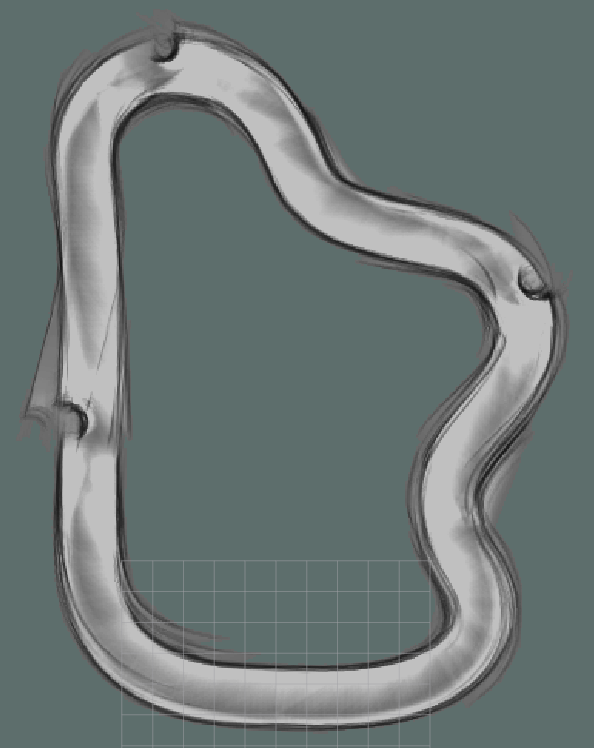
\includegraphics[width=\textwidth]{Pictures/3slamtest4}
		\caption{\nth{4} round}
	\end{subfigure}
	%\hskip2em
	\begin{subfigure}{.3\linewidth}
		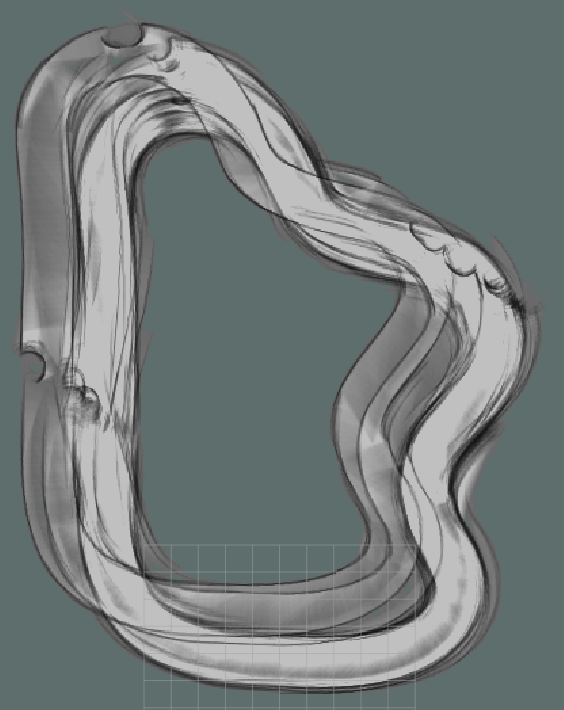
\includegraphics[width=\textwidth]{Pictures/3slamtest10}
		\caption{\nth{10} round}
	\end{subfigure}

	\caption{Slam Map rounds during long duration test}
	\label{4slamtest}

\end{figure}

As pictured in \ref{4slamtest} cartographer struggles with aligning the submaps during obstacle avoidance and suffers from rotational error.\\
Fortunately these errors are mostly corrected over the period of the next few rounds.\\ In the \nth{10} round however cartographer suffers from the same issue highlighted by the long duration test. Here it is clearly visible, that the queue of unmatched submaps is more than one entire round.\\

\textbf{Discussion of the test results}\\
As proven by the first two tests, cartographer is well tuned and the map would be useable for goal extraction. The submaps are well alligned and the map has no huge translational or rotational offset.\\

The \nth{3} and \nth{4} test on the other hand display the limitations of the slam algorithm in this use case.\\
When obstacles are located on the right lane the allignment of the submaps fails and a lot of submaps cant be attached to the rest of the map. After passing the same obstacle in multiple rounds the map improves to a point where it would be usable for goal extraction.\\
The \nth{3} test proves that cartographer is not usable in SLAM mode during long time navigation an a circuit. This is caused by the amount of submaps that are close to each other and the resulting amount of constraints between each of them.\\

Based on these test results it is not feasible to use the SLAM map for navigation with obstacles on the road, since the map is just not reliable enough.




\section{complete system test}
The following subsections cover the discussion of the complete system tests.\\
\textbf{No obstacles}\\
The reasoning for this test is, to check how good the robot stays on the right lane. Therefore the robot drives in the described test environment, while the difference between the right lane and the robot center is monitored.

\begin{figure}[H]
	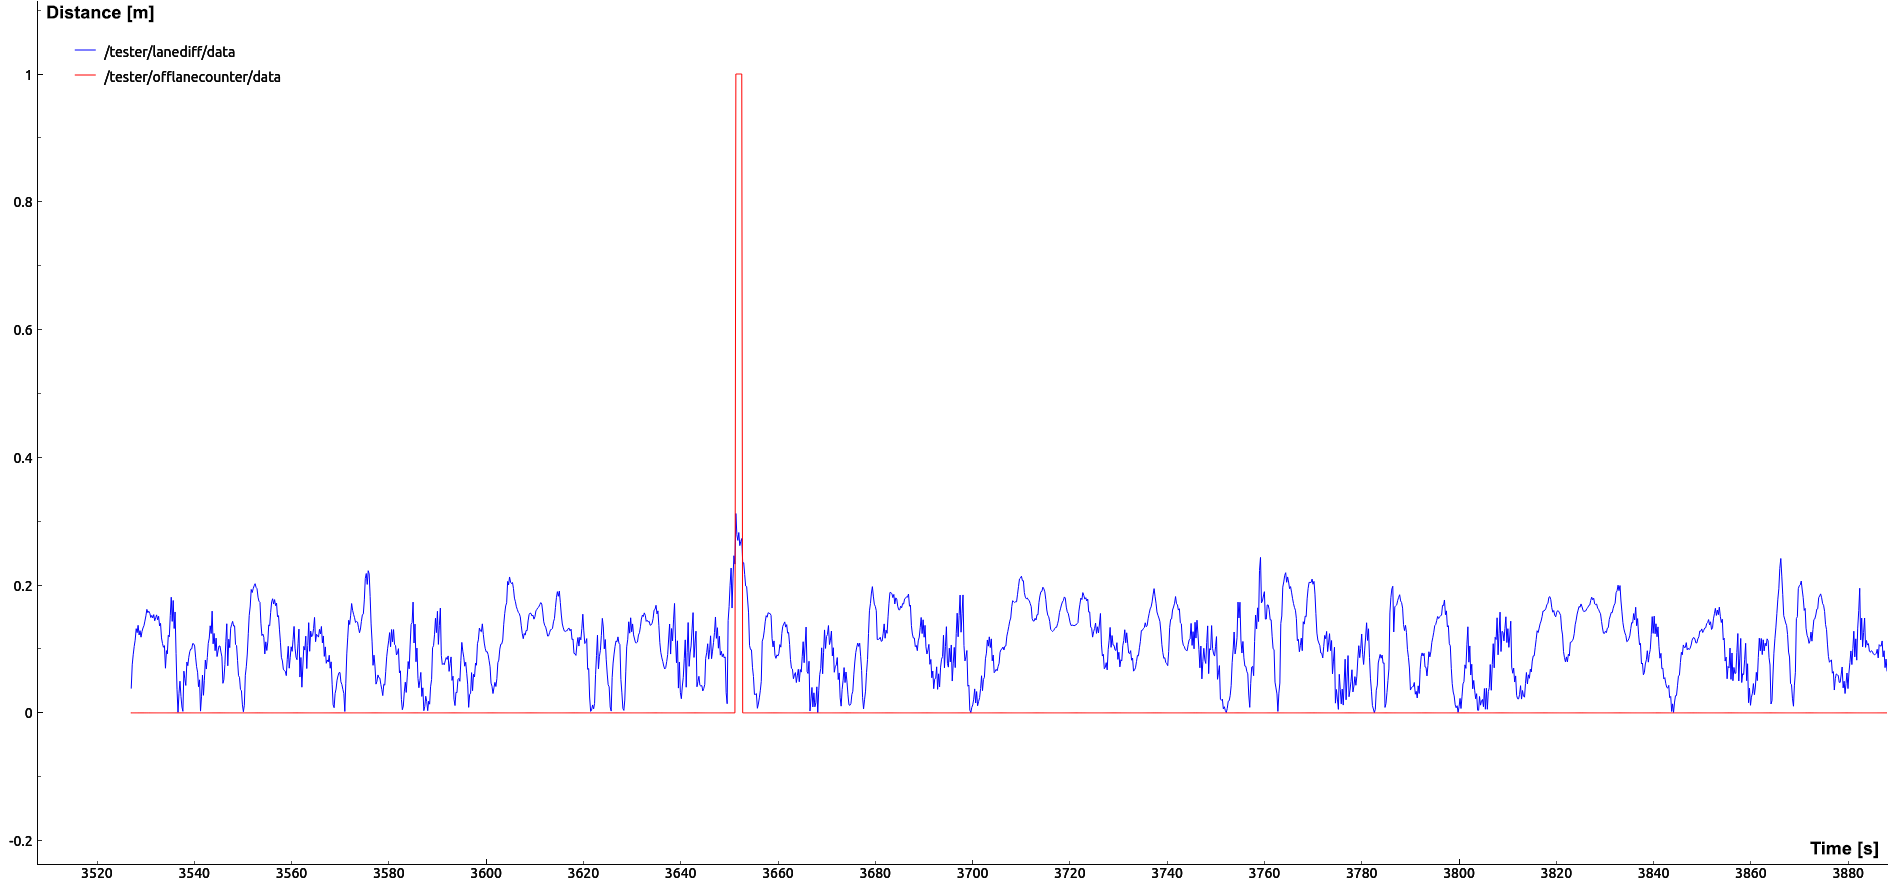
\includegraphics[width=\textwidth]{Pictures/final analysis no obstacle}
	\caption{absolute error of the robot trajectory and rectified signal of the avoidance duration}
	\label{noobserr}
\end{figure}

As pictured in \ref{noobserr} the robot has left the road markings once.\\

\begin{figure}[H]
	\begin{subfigure}{.5\linewidth}
		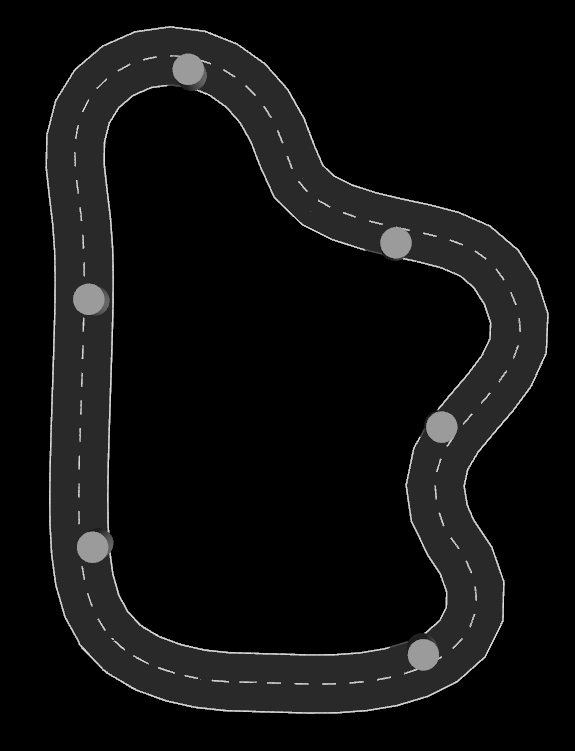
\includegraphics[width=\textwidth]{Pictures/obstacle left final 2}
		\caption{obstacles on left lane}
	\end{subfigure}	
	%\hskip2em
	\begin{subfigure}{.5\linewidth}
		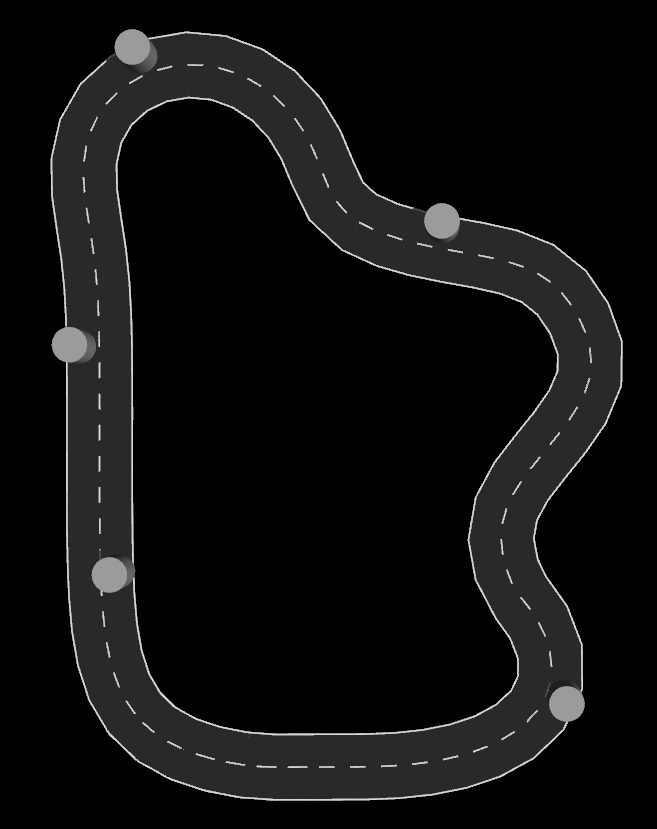
\includegraphics[width=\textwidth]{Pictures/right final obs}
		\caption{obstacles on right lane}
	\end{subfigure}

	\caption{Obstacle placement for both final tests}
	\label{obstaclefinaltest}

\end{figure}
\textbf{Obstacles on left lane}\\
This test is supposed to test the behavior of the navigation when obstacles block the view of the camera but the robot has to drive on the right side. In this test the robot will not drive as many rounds, since the goal is to observe the behavior when passing goals. In contrast to Figure \ref{noobserr} the distance to the nearest obstacle will be included in the graph, thus it can be determined, if the robot left the lane because it is near an obstacle or not, for this the true positions from the simulation will be used. The obstacle distance will only be tracked, if it is below 3 meters.
\begin{figure}[H]
	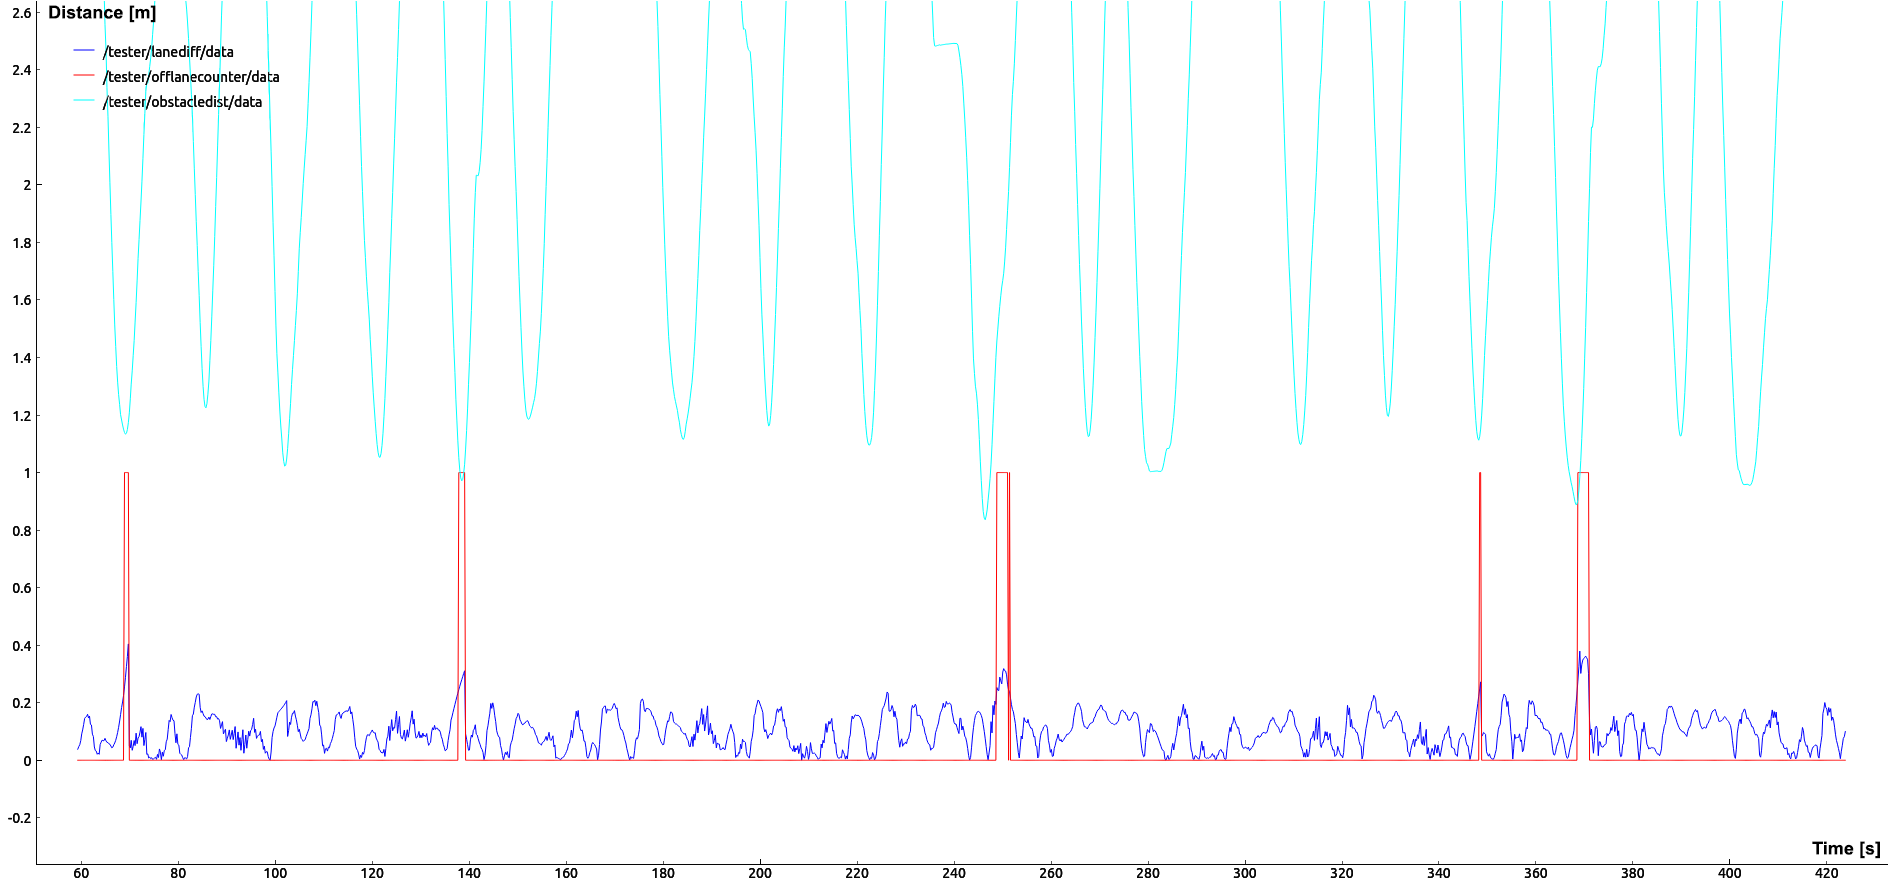
\includegraphics[width=\textwidth]{Pictures/left obs final obs2}
	\caption{graph of left lane obstacle test}
	\label{leftobsfinal}
\end{figure}
As visible in figure \ref{leftobsfinal} the robot left the right lane way more often compared to \ref{noobserr}.\\

\textbf{Obstacles on right lane}\\

To cover the possible scenarios of the carolo cup this test is supposed to be a realistic application with a few obstacle scattered over the entire environment on the right lane. Like in the last test the obstacles will be located as well in corners, as on straight sections of the road.

\begin{figure}[H]
	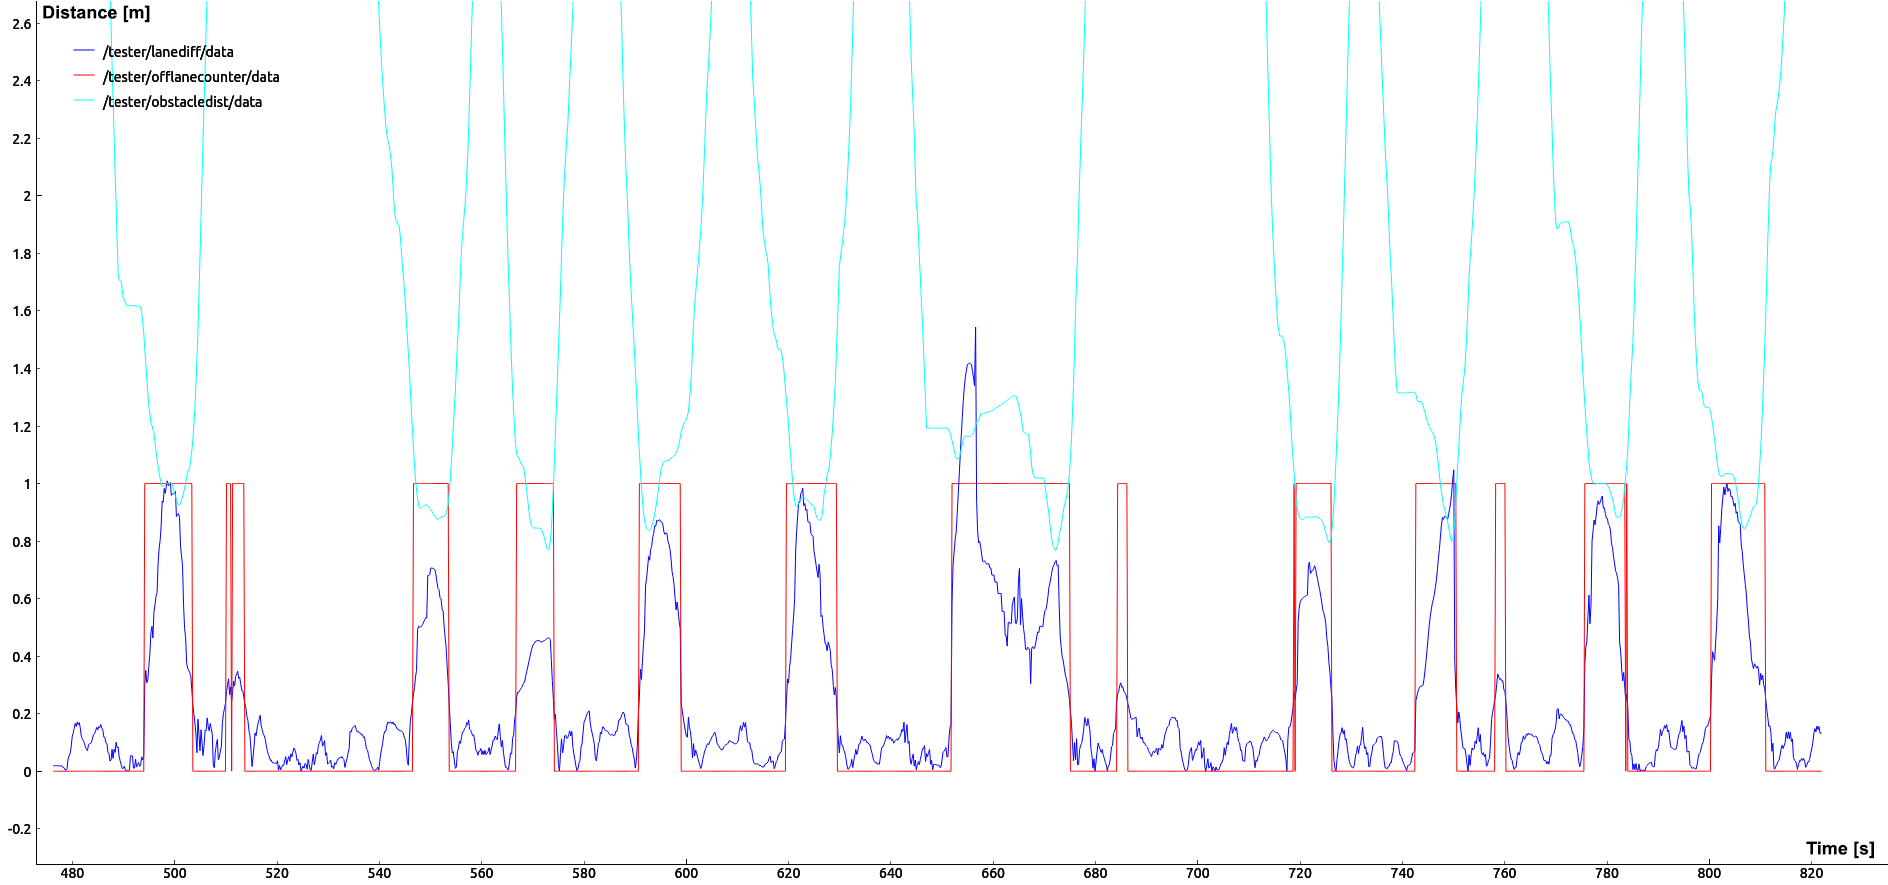
\includegraphics[width=\textwidth]{Pictures/right obs final obs}
	\caption{graph of right lane obstacle test}
	\label{rightobsfinal}
\end{figure}


As pictured in Figure \ref{obstaclefinaltest}, there are five obstacles on the right lane. These can be seen, when inspecting the graphe in Figure \ref{rightobsfinal}, which shows two rounds of the robot.

Furthermore the graph shows, that the robot successfully avoided all obstacles in both rounds. Unfortunately the robot left the lane three times, when no obstacle in the proximity of it.\\

In the middle of the graph the robot took particularly long for the avoidance.

The graph also shows, that the avoidance is all ways finished before the robot is two meters away from the obstacle and therefore satisfies this condition.

\subsection{Discussion}

The results of the complete system tests show, that the navigation performs really well during simple lane following, since the road detection recognizes the road almost allways as shown in the road\_detection test.

While observing the robot during driving past obstacles on the left lane it was noticeable, that the robot mostly left the lane, directly after it passed an obstacle in or directly after a corner.\\ 
In this case the predicted goal pulls the robot into the middle of the road, since the costmap does not yet have information about the road and therefore will not force the global plan to the right lane. The approximated goal is still constructed with the circle approximation since the upcoming straight section has net yet been seen.\\

Obstacle avoidance suffers from a similar problem. As shown in the \nth{3} test. Here it is visible, that the robot passes the obstacle nicely, but after passing drives along the center of the road, which causes the spikes of the rectified signal visible in \ref{rightobsfinal} after the ovoidance. As soon as the robot has passed an obstacle fully it drives straight to the predicted goal while waiting on new data from the road\_detection, which often causes unnecessary long avoidance periods.





